% Figure: the network ensemble interpolated between bin centres, against the smooth model.
\begin{figure}[t]
\centering
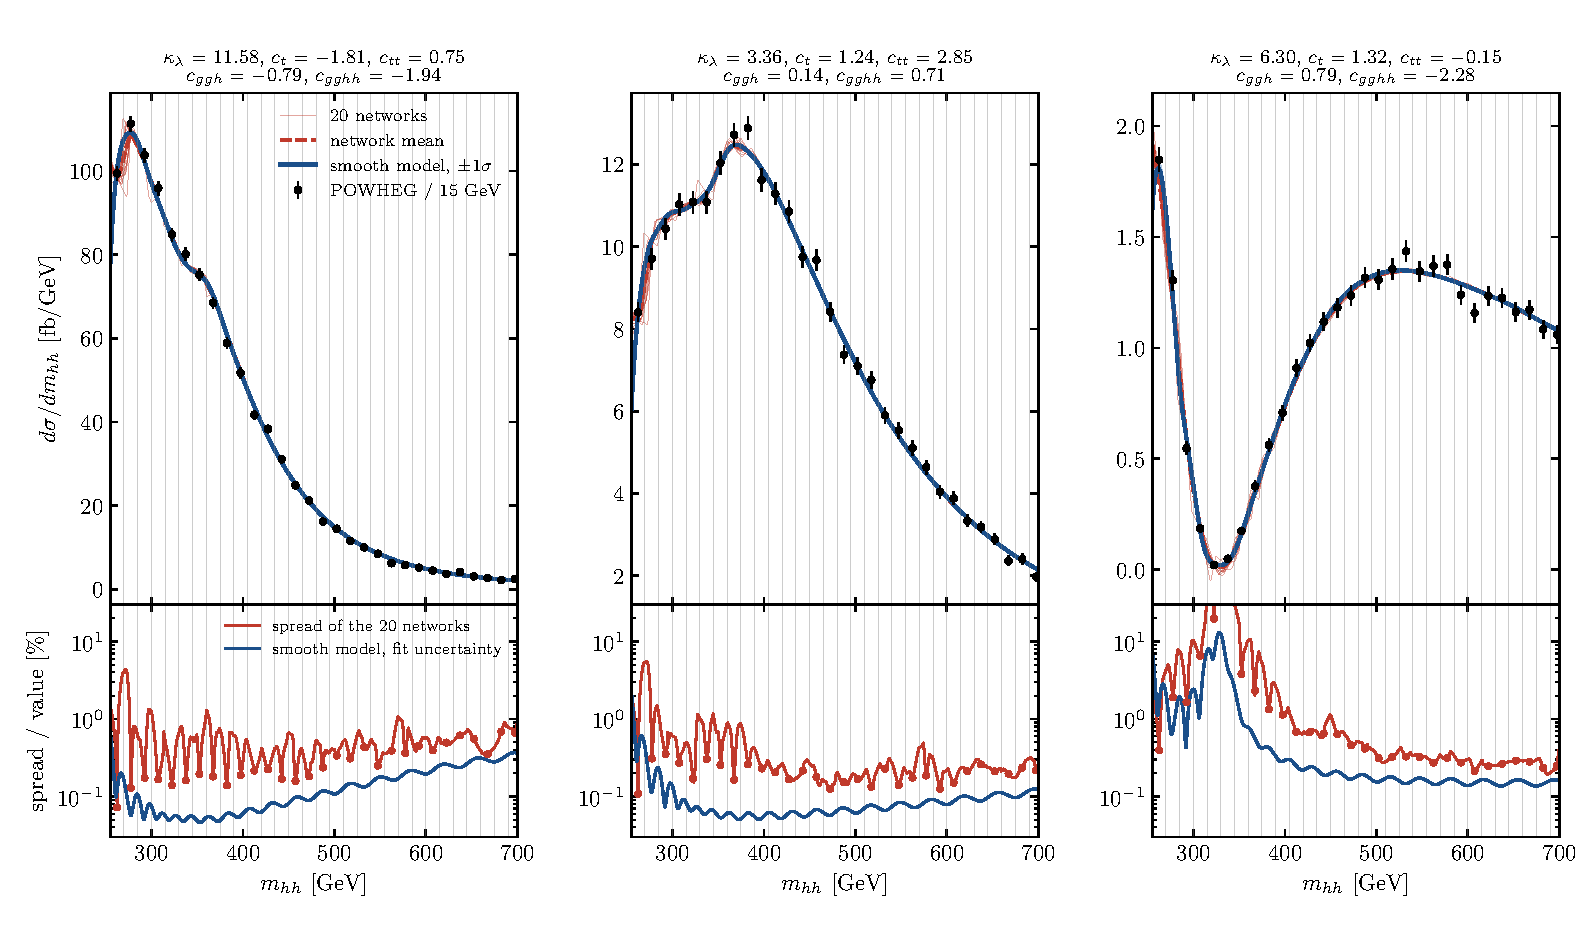
\includegraphics[width=\textwidth]{fig_interpolation.pdf}
\caption{Interpolating between the bin centres, for the three median test spectra of
figure~\ref{fig:spectra}, below 700~GeV. Top: the 20 fine-tuned networks (thin red lines) and
their mean (dashed), evaluated on a 0.5-GeV grid and divided by the 15-GeV bin width; the
smooth model's density with its $\pm1\sigma$ fit uncertainty (blue); POWHEG divided by the bin
width (points). Vertical lines mark the bin edges. Bottom: the relative spread of the 20 networks
(red; dots at the bin centres) and the relative fit uncertainty of the smooth model (blue). The
networks were trained only at the 80 bin centres: their spread is smallest there and grows
between them, by more than an order of magnitude near threshold, whereas the smooth model, fitted to the bin
integrals, is constrained across every bin.}
\label{fig:interpolation}
\end{figure}
